%Description: Thesis template that matches the
% Mid Sweden University thesis Word template.

% Author: Linus Sjöbro
\documentclass[12pt]{report}
% Basic settings
% ---------------------------
\usepackage[utf8]{inputenc}
\usepackage[english]{babel}
\usepackage[%
top=4.47cm,
bottom=3.64cm,
left=3.7cm,
right=3.7cm,
headheight=50pt
]{geometry}

\usepackage{minted}
\usepackage[yyyymmdd]{datetime}
\renewcommand{\dateseparator}{--}

% Font and text manipulation
% ---------------------------
\setlength{\parindent}{0em}
\renewcommand{\baselinestretch}{1.2}
\usepackage{mathpazo, helvet}
\usepackage{titlesec}


% Move section numbering into the margin
\makeatletter
\def\@seccntformat#1{\rlap{\hskip-50pt\csname the#1\endcsname}}
\makeatother

\titleformat{name=\chapter, numberless}
  {\sffamily\LARGE\bfseries}{}{2.3em}{}
  \titlespacing*{\chapter}{0em}{-1em}{0em}

% Place chapter number and name on same row and change margins
\titleformat{\chapter}
  {\sffamily\LARGE\bfseries}{\thechapter}{1.8em}{}
  \titlespacing*{\chapter}{-50pt}{-1em}{0em}

\titleformat{\section}
  {\sffamily\Large\bfseries}{\thesection}{1.45em}{}
  \titlespacing*{\section}{-50pt}{1em}{0em}

\titleformat{\subsection}
  {\sffamily\large\bfseries}{\thesubsection}{1.25em}{}
  \titlespacing*{\subsection}{-50pt}{1em}{0em}
  
\titleformat{\subsubsection}
  {\sffamily\normalsize\bfseries}{\thesubsubsection}{0.8em}{}
  \titlespacing*{\subsubsection}{0em}{1em}{0em}

\titleformat{\paragraph}[runin]
  {\sffamily\normalsize\bfseries}{\theparagraph}{1em}{}
  % \titlespacing*{\subsubsection}{-50pt}{1em}{1em}

% Header
% ---------------------------
\usepackage{fancyhdr}
\fancypagestyle{plain}{
    %Deletes the original header and footer
    \fancyhf{}
    
    \fancyhead[L]{\textsf{\thesisTitle \\ \thesisAuthor}}
    \fancyhead[R]{\textsf{\today}}
    
    \fancyfoot[C]{\thepage}
}
\pagestyle{plain}



% Bibliography
% ---------------------------
\usepackage[
    backend=biber,
    style=ieee,
    sorting=none
]{biblatex}

\usepackage{csquotes}
\addbibresource{bibliography.bib}


% Figures and drawings
% ---------------------------
% Drawings
\usepackage{tikz}
\usetikzlibrary{calc}

% Misc
% ---------------------------
\usepackage{microtype}
% \usepackage{nameref}

% Hyperlinks for URL's and table of content
\usepackage[bookmarks]{hyperref}

\usepackage{float}


% Glossaries
% ---------------------------
\usepackage[acronym, nopostdot, section]{glossaries}
\makeglossaries
\newacronym{ble}{BLE}{Bluetooth Low Energy}
\newacronym{ar}{AR}{Augmented Reality}
\newacronym{poc}{PoC}{Proof Of Concept}
\newacronym{ux}{UX}{User experience}
\newacronym{ui}{UI}{User interface}
\newacronym{rssi}{RSSI}{Received Signal Strength Indication}
\newacronym{knn}{K-NN}{K-Nearest Neighbour}
\newacronym{ann}{ANN}{Artificial Neural network}
\newacronym{svm}{SVM}{Support Vector Machine}
\newacronym{ap}{AP}{Access Point}
\newacronym{ips}{IPS}{Indoor Positioning System}
\newacronym{json}{JSON}{Javascript Object Notation}
\newacronym{uuid}{UUID}{Universally unique identifier}




% Appendix
% ---------------------------
\usepackage[toc, page]{appendix}
% \renewcommand\appendixtocname{Bilagor}
% \renewcommand\appendixpagename{Bilagor}
% \AtBeginEnvironment{appendices}{\renewcommand\thesection{\Alph{section}}}


% Better references in the document
\usepackage[noabbrev]{cleveref}
\AtBeginEnvironment{appendices}{\crefalias{section}{appendix}}


% Imports from other files
% ---------------------------
% Custom commands for cleaner and
% easier implementation in the document.

\newcommand{\fig}[4]{%
    \begin{figure}[H]
        \centering
        \includegraphics[width=#3\textwidth]{#4}
        \caption{#1}\label{fig:#2}
    \end{figure}
}

\newcommand{\framedFig}[4]{%
    \begin{figure}[H]
        \centering
        \framebox{\includegraphics[width=#1\textwidth]{#3}}
        \caption{#4}\label{fig:#2}
    \end{figure}
}

\newcommand{\fileListing}[4]{%
    \begin{listing}[H]
        \caption{#1}
        \label{listing:#2}
        \inputminted[frame=lines]{#3}{\codePath #4}
    \end{listing}
}

\newcommand{\fileListingNoCap}[2]{%
    \begin{listing}[H]
        \inputminted[frame=lines]{#1}{\codePath #2}
    \end{listing}
}

\newcommand{\tikzFig}[2]{%
    \begin{figure}[H]
        \centering
        \resizebox{1\textwidth}{!}{%
            \input{\tikzPath #1.tex}
        }%
        \caption{#2}\label{fig:#1}
    \end{figure}
}

\newcommand{\texTable}[3]{%
    \table[H]
        \centering
        \caption{#1}\label{tab:#2}
        \input{\tablePath #3.tex}
    \endtable
}

\newcommand*{\fullref}[1]{\textit{\cref{#1} \nameref{#1}}}
\newcommand*{\Fullref}[1]{\textit{\Cref{#1} \nameref{#1}}}


\graphicspath{{./attachments/figures/images/}}
\newcommand{\codePath}{./attachments/code/}
\newcommand{\tikzPath}{./attachments/figures/tikz/}
\newcommand{\tablePath}{./attachments/tables/}

\newcommand{\thesisTitle}{Automatic presentation of data for industrial machines with hand held devices}
\newcommand{\thesisSubtitle}{Positioning in indoor environments without GPS-signals}
\newcommand{\thesisAuthor}{Linus Sjöbro}

\newcommand{\examinerName}{Mårten Sjöström}
\newcommand{\supervisorName}{Roger Olsson}
\newcommand{\degreeProgramme}{Master of Science in Engineering: Computer Engineering, 300 hp}
\newcommand{\courseCode}{DT005G}
\newcommand{\courseCredits}{30 hp}
\newcommand{\mainFieldOfStudy}{Computer science}
\newcommand{\thesisYear}{2021}
\newcommand{\semester}{spring}


\begin{document}
\thispagestyle{empty}
\pagenumbering{roman} 
\setcounter{page}{2}
\sffamily
\begin{titlepage}
  \setlength\headheight{59pt}
  \renewcommand{\headrulewidth}{0pt}
  \thispagestyle{fancy}
  \fancyhf{}
  \rhead{
\includegraphics[width=41mm]{settings/images/miunLogo.jpg}}
  \fancyfoot{}

  \vspace*{0.5cm}
  {\fontfamily{phv}\selectfont{%
    \Huge{\textbf{\thesisTitle}}}
    \\
    \\
    \Large{\thesisSubtitle}
    \\
    \\
    \\
    \Large{\thesisAuthor}
  }

  \vspace*{11cm}
  \begin{tabular}{l}
    \footnotesize{Main field of study: \mainFieldOfStudy}\\
    \footnotesize{Credits: \courseCredits}\\
    \footnotesize{Semester/Year: \semester, \thesisYear}\\
    \footnotesize{Supervisor: \supervisorName}\\
    \footnotesize{Examiner: \examinerName}\\
    \footnotesize{Course code: \courseCode}\\
    \footnotesize{Degree programme: \degreeProgramme}
  \end{tabular}
\end{titlepage}

\newpage
\chapter*{Abstract}
\addcontentsline{toc}{chapter}{Abstract}
Positioning of mobile phones or other handheld devices in indoor environments is hard because it's often not possible to retrieve a GPS-signal.
Therefore, other techniques need to be used for this.
Despite the difficulties with indoor positioning, the Swedish mining company LKAB want to do exactly this in  their production plants.
LKAB has developed an Apple iPhone mobile application to maintain real-time process data and documents for a machine.
But to retrieve the information an OCR code need to be manually scanned with the application.
Instead of manually scanning these codes, LKAB want to develop an \acrlong{ips} that can automatically locate handheld devices in their production plants.
This thesis aimed to create a \acrfull{poc} Apple iOS application that can position devices without GPS-signals.
In the system developed \acrlong{ble} iBeacons is used to transmit data to the application.
From this data \acrlong{rssi} values is  collected and sent off to a server that transform the values into positioning fingerprints.
These fingerprints are used together with the classification algorithms \acrlong{knn} to determine in which, on pre-hand created, group the user is located.
In these created groups there is a defined set of machines that is being presented back to the user.
Test results conducted with the \acrshort{poc} application shows that the implemented system works and gives a positioning accuracy up to 75\%.


\bigskip

\textbf{Keywords:} RSSI, KNN, fingerprints, indoor positioning, Apple, iOS, application, iBeacon, Beacon

\chapter*{Acknowledgements}
\addcontentsline{toc}{chapter}{Acknowledgements}
I want to thank my supervisor at Mid Sweden University, Roger Olsson, for the help under this project and for the very clear and good feedback, in both the work and to get a better written report.
This has helped me a lot.

\bigskip

I would also want to thank LKAB and my supervisor at the company, Stefan Karlström, to trust in my work and giving me the opportunity to conduct this thesis work at them. 
They did also provided me with hardware and software needed to perform the thesis.





\tableofcontents

\listoffigures
\addcontentsline{toc}{chapter}{List of Figures}

\listoftables
\addcontentsline{toc}{chapter}{List of Tables}

\chapter *{Terminology}
\addcontentsline{toc}{chapter}{Terminology}
% \printglossary[title = Words, nonumberlist]
\printglossary[title=Acronyms, type=\acronymtype, nonumberlist]

\chapter{Introduction}\label{sec:intro} \pagenumbering{arabic}

\section{Background and problem motivation}\label{sec:introBackground}
The Swedish mining company LKAB has devveloped
a smartphone application, named InfoHub, that will help their mechanics and
technicians.  This application is capable to shows real time data and documents
for a chosen type of machinery out in their iron ore production plants.  To
choose which machine to show data from a onsite OCR code need to be manually
scanned in the application.  Due to the harsh and dirty environment in these
production plants the application could face difficulties reading these codes.
The manual scanning also means that the user must know the location of the code,
which sometimes could be hard to find.

\bigskip

A better way to get the information for a machine is to automatically fetch the
process data when the user is standing nearby.  This could be done by knowing
the users position in the production plants and display the corresponding data
to the user.  This is happening in indoor environments where there is no access
to GPS signals.  This means that the positioning need to be done with other
techniques such as WiFi or \acrlong{ble} Beacons.

\bigskip

When a user scan a verifiable code the application will fetch the documents and
real time data for the machine that matches the code.  The application gets the
data from Microsoft's Azure cloud services that is being uploaded from LKAB's
local onsite systems.


\section{Overall aim}\label{sec:introOverallAim}
The overall aim in this thesis work is to investigate and implement a proof of concept solution for indoor non GPS positioning for LKAB's specific needs and environment.
The purpose with the positioning is to be able to skip the manual OCR code scanning step in the InfoHub application.


\section{Problem statement}\label{sec:introProblemStatement}
The problem statement in this thesis work is stated as follow: How, as accurate as possible, locate handheld devices in indoor environments without any GPS signal?


\section{Verifiable goals}\label{sec:introGoals}
\begin{enumerate}
\item \label{goal:posInvestigation}
Investigate how to achieve a high indoor positioning resolution without GPS
techniques in LKAB's production plants environments, where WiFi-networks has
not yet been fully deployed.

\item \label{goal:poc}
Develop a \acrfull{poc} Apple iOS application that implement the resulting
positioning technique from knowledge goal \ref{goal:posInvestigation}. This
implementation should result in;
\begin{itemize}
\item Measurable result in form of resolution and location accuracy
\end{itemize}
\end{enumerate}


\section{Scope}
The focus in the positioning area will be to only position smartphone devices at one floor plan.
The proof of concept system will therefore not take multiple floor plans into consideration.
The system will be tested in a office environment and not in any of LKAB's production plants due to
limitations in testing areas.


\section{Outline}

\chapter{Theory}\label{theory}
This chapter presents the theoretical part is this work.
It starts with an explanation of the company LKAB, followed by 
different techniques used to position a device without access to GPS-signals.

\section{LKAB}
Luossavaara-Kiirunavaara AB (LKAB) is a high tech iron ore and mineral mining company with its base in northern Sweden established year 1890.
LKAB is operating in twelve countries over the world with a total of 4300 employees.
Iron ore is their main area which is being mined and processed in Sweden.
Other areas in the company are industrial minerals, drilling systems, rail transport, rockwork services and property management.
In 2019 LKAB produces 27 million tonnes of iron ore products, with a net sales amount of 31 billion SEK. \cite{LKABBrief} 

\bigskip

LKAB stands in front of one of the largest industrial investments ever in Sweden.
An investment of between 10 and 20 billion SEK that extends over more than 20 years and will create between 2000 and 3000 new jobs opportunities.
This investment will result in carbon-dioxide-free iron ore products. \cite{LKABInvestment}

\bigskip

LKAB was the first underground mine with wireless connectivity and today has the largest underground WiFi-network in the world.
With LKAB 5.0 all vehicles and personnel will be connected to these WiFi-networks.
This shows that the company has a high digitalization maturity. \cite{LKABITDevelopment}

\bigskip

The productions plants needs constant maintenance and overseeing to be fully functional.
Due to the large number of machines and the complexity of certain machines it's hard to service them without any additional help.
LKAB has developed an Apple iOS application called Infohub that help the employees out in the productions plants to show real-time process data and documentation.


\section{Received Signal Strength Indication}\label{sec:theoryRssi}
\acrfull{rssi} is an indication of the signal strength between a sender and receiver.
It's a less complex method than other technologies such as Time of Arrival, Time Difference of Arrival or
Angle of Arrival that require a proper time synchronization between the sender and receiver.
The benefits with \acrshort{rssi} based measurements is that it will reduce the complexity of the signal measurement, and opens up for easier software implementations.
It does also have a high accuracy, low power consumption and a low cost due to the less complex systems required.
It became a popular choice to use in non GPS-based positioning because of these benefits.\cite{IndoorFingerprintPositioning2017} 

\bigskip

\acrshort{rssi} measurements can be divided into three different categories;

\begin{itemize}
	\item Trilateration
	\item Approximate Perception
	\item Scene Analysis \cite{IndoorFingerprintPositioning2017}
\end{itemize}

\subsection{Trilateration}\label{sec:theoryRssiTrilateration} Trilateration
is a positioning technique where three or more senders and receivers converts the signals
into spatial distances.  This is used to create radius of circles and where all
the circles intersect with each other is where the device is located.
\cite{IndoorFingerprintPositioning2017} 

\bigskip

The radio frequency can easily be affected because of the complexity of the indoor space, which will impact the signals from the transmitters.
In the conversion from signal strength to spatial distances it can therefore introduce errors that will lower the accuracy of the positioning.
A solution to assist the technique is path loss models that will increase the accuracy.
Since spatial distances is used to position a device, the exact position of the WiFi \acrfull{ap} need to be known. 
Together with this exact position and the path loss models the technique is not practical to use, and also has a low positioning accuracy of around 40 meters.\cite{IndoorFingerprintPositioning2017}


\subsection{Approximate Perception}\label{sec:theoryRssiApproxPerception}
In approximate perception the signal from the strongest base station is the positioning criterion.
Positioning with this technique requires information of the base stations location as well as the area they cover. 
This technique has a low positioning accuracy, or around 100 meters, and to make it more precise researchers has used a cluster of antennas.
This cluster is then placed at a know location and will improve the accuracy.
\cite{IndoorFingerprintPositioning2017} 

\subsection{Scene Analysis}\label{sec:theoryRssiSceneAnalysis}
Scene analysis is the most used technique for indoor positioning.
It uses fingerprint matching (\cref{sec:theoryFingerprint}) and does not require any information of where the base stations is located, which is needed in both trilateration and approximate perception.
The positioning is done with the signal strength from multiple base stations at a given reference point.
Together with a fingerprint data structure, the reference point will act as a localization point for the positioning system.\cite{IndoorFingerprintPositioning2017} 

\bigskip

Measurements based on transmitters \acrshort{rssi} values can be used to make signal fingerprints to build up a radio map database that will position the device.\cite{DevelopmentMobileIndoor2017} 

\section{Positioning fingerprint}\label{sec:theoryFingerprint} A position fingerprint is a popular method for indoor positioning systems. 
Fingerprint positioning can be used both for indoor and outdoor positioning.
Indoor positioning is based on 2D modelling where positioning via WiFi Access Points (AP) is the most popular alternative.
For indoor positioning the fingerprints are often based on \acrshort{rssi} values from the sending devices for every location.
\cite{LocationFingerprintingInfrastructure2004,
IndoorFingerprintPositioning2017}

\bigskip

Fingerprint based localization is not only used in WiFi based systems but can
also be used with other hardware, such as \acrshort{ble} Beacons (\cref{sec:theoryBleiBeacons}).
\cite{PracticalFingerprintingLocalization2017} 

\bigskip

A fingerprint positioning system is built up in a two phase process.  An offline
and online phase.\cite{IndoorFingerprintPositioning2017} 

\subsection{Offline phase}\label{sec:theoryFingerprintOffline} In the offline
phase (also called observation phase) the fingerprints are being collected and
mapped to a location in the environment.
The mapped fingerprints are then being stored in a radio map database.
\Cref{fig:fingerprintOfflinePhaseIllustration} shows the flow for collecting the \acrshort{rssi} signals, mapping them to a location and storing them in the radio map database.  This is often an time consuming part since all positions need to be manually
scanned.\cite{IndoorFingerprintPositioning2017} 


\fig{Fingerprint offline phase flow \cite{IndoorFingerprintPositioning2017}
}{fingerprintOfflinePhaseIllustration}{1}{fingerprintOfflinePhase}


\subsection{Online phase}\label{sec:theoryFingerprintOnline} The online phase
is the part where a user is interacting with the stored fingerprints.
A device is collecting \acrshort{rssi} values from nearby senders in real time.
These collected values is then being compared with the fingerprints in the database.
If a match between the real time \acrshort{rssi} values and the radio map occur the location is being yield back and the device can be positioned.
\Cref{fig:fingerprintOnlinePhaseIllustration} show a illustration of the
online phase.
\cite{IndoorFingerprintPositioning2017}

\fig{Online phase positioning flow\cite{IndoorFingerprintPositioning2017}
}{fingerprintOnlinePhaseIllustration}{1.0}{fingerprintOnlinePhase}


\section{Bluetooth Low Energy}\label{sec:theoryBle}
The wireless technology \acrfull{ble} is part of the core specifications of Bluetooth 4.0 and is also referred as Bluetooth Smart.
\acrshort{ble} focuses on short-range communication where the transmission strength often is measured in dBm.
A closer distance between the receiver and transmitter means a lower dBm-value, which typically range between around -30 dBm to 0 dBm.
\cite{DevelopmentMobileIndoor2017} 

\bigskip

\acrshort{ble} technology is designed to be used where the devices doesn't need to transmit a lot of data.
With this comes a low power consumption and often low cost, which makes \acrshort{ble} a good candidate for a various of different tasks.
\cite{PracticalFingerprintingLocalization2017} 


\subsection{iBeacons}\label{sec:theoryBleiBeacons}
iBeacon are small battery powered devices developed by Apple that is based on the existing \acrshort{ble} technology.
Using the iBeacon technology together with the Apple iOS platform open up for a variety of opportunities when in comes to implementing position based applications.
Because of the small footprint and low cost of these devices they are easy to deploy in an environment where they can be used together with a smartphone application.
\cite{BluetoothLowEnergy2018} 

\bigskip

The iBeacon is sending out an advertise signal that consists of three parts;
\begin{itemize}
\item 16-byte UUID
\item 2-byte major value
\item 2.byte minor value \cite{GettingStartedIBeacon2014} 
\end{itemize}

The UUID value is a fixed identifier that will identify a set of beacons.
This value needs to be the same for all the beacons that will be used.
The major value is used to identify a large set of beacons with the same UUID, and the minor value is used to identify a specific beacon.
\cite{GettingStartedIBeacon2014}

\bigskip

An example of the iBeacon deployment mentioned in \cite{GettingStartedIBeacon2014} is a global retail store. The UUID will be the same for all stores, meanwhile the major value is used to identify a specific store and the minor value to identify a department in each of the stores.
\cite{GettingStartedIBeacon2014} 


\section{Instance-based learning}\label{sec:theoryInstanceLearning}
Instance-based learning is a set of algorithms within data mining and machine learning and is often referred as lazy classification.
In the training phase the algorithms does not require much work since it is being trained on already stored instances.
\cite[p. 78]{DataMiningPractical2011} 

\bigskip

The real work is done when a new instance is being classified.
This new instance is compared to all other, already stored, instances. 
The comparison between a new instance and the stored ones is being classified with a distance metric, where the closest, already stored, instance is used to assign a class to the new one.
This classification method is called nearest-neighbour classification, and when being compared to \textit{k} neighbours it's called k-nearest-neighbour.
\cite[p. 78]{DataMiningPractical2011} 

\bigskip

With instance-based learning new examples can be inserted into the training set at any time.
Which means that the training set can be extended with new data as the number of data points groves larger.
\cite[p. 135]{DataMiningPractical2011} 


\subsection{K-Nearest Neighbour}\label{sec:theoryUnClassKnn}
In \acrfull{knn} classification a data instance is being compared to a set $k$ of its nearest neighbours.
These neighbours are like in general instance-based learning previously stored instance that are being used to compare against.
The method is perfectly suited when this new instance need to be classified \cite[p. 77-79]{DataMiningPractical2011}

\bigskip

If a set of one numeric values are compared the computation of the distance between the two points are trivial. 
It only computes the difference between these two values.
With two or more values the computation is almost as straightforward.
In these cases, the Euclidean Distance method (which is the default) is used to make the computation and comparison of the values.
An important part is that the data need to be normalized and of equally importance.
One of the problems in the learning phase is to determine the important values.
\cite[p. 77-79]{DataMiningPractical2011}

\bigskip

\Cref{fig:knnIllustration} illustrates a representation when a new instance is being classified into an already existing set or area.
The green and red dots are already existing instanced, and the blue dot is new and is going to be classified.
In this case the new instance is going to be classified as red, if $k=3$.

\fig{KNN classification of a new instance where $k=3$}{knnIllustration}{0.3}{knnClassification}

% \bigskip

% The K-value need to be uneven to make the classification as good as possible. 
% In cases where $k$ is even a condition where the new instance is equally between two areas can occur.
% Which will lead up to a lower accuracy, since one of the areas need to be chosen.


\section{Related work}\label{sec:theoryRelatedWork}




\chapter{Method}\label{method}

\fig{Method overview}{methodOverview}{1}{methodFlow}


\section{Research strategy}\label{sec:methodResearch}
This chapter will present and motivate the chosen research strategy.

\subsection{Case study}\label{sec:methodResearchCaseStudy}
The research strategy in this thesis work was a case study aimed to the company
LKAB, which wanted to see the possibilities how indoor positioning could be
designed.







\chapter{Implementation}\label{impl}
This chapter describes the details about the development of the \acrfull{poc} application that's being implemented to meet requirement number \ref{req:developeApp} presented in appendix \ref{appendix:requirements} and to fulfil goal \ref{goal:poc} (\cref{sec:introGoals}).

\section{Architecture}\label{sec:implArchitecture}
To fully understand the implementation of this project some architectural descriptions is needed.
This section will present different techniques and architectures used in this implementation.


\subsection{Machine}\label{sec:implArchitectureMachine}
A machine is being defines as some kind of equipment places around a industrial hall in an manufacturing environment.
This could for example be a waterpump or electrical engine that drives a stone crusher.
A machine in this work it only a set of data collections in a database and not a real physical machine.


\subsection{Group}\label{sec:implArchitectureGroup}
A group in the system is what's being located with the positioning.
The system sets up invisible boundaries in an undefined spaced out in a production hall.
When a device is being located by the system a group will be yield back instead of a physical exact position.
Machines are tied to these created groups where the machines data will be shown when the group is positioned.


\subsection{Device}\label{sec:implArchitectureDevice}
A device refer to a mobile hand held device that's in this work is an Apple iPhone 12 pro.
This device is running the developed application.


\subsection{Beacons}\label{sec:implArchitectureBeacons}
A beacon, also mentioned as iBeacon is the transmitting hardware used to position a device with the developed system.


\subsection{Server}\label{sec:implArchitectureServer}
All calculations are being taken care of by a server.
This server is not being hosted to any cloud service or a physical server in a data centre, instead it is running on a local computer where the device will communicate with the server only in the same LAN.


\subsection{Frontend vs. backend}\label{sec:implArchitectureFrontBack}
In the developed \acrshort{ips} there are two major parts, a front- and backend.
The application is defined as the frontend of the system since this is the part that a user will interact with and get data presented to it. 
The backend is the developed server software that takes care of all calculations and data predictions, and delivers this to the frontend.


\subsection{API}\label{sec:implArchitectureApi}
An API is the data connection between a device and a server.
Data it sent from the device to the server via specific API \textit{endpoints} that is being defined in the application and created in the server.
The developed API works with two different types of requests, POST and GET.

\bigskip

In a POST request the device is giving some kind of data to the server that will be processed.
When the server is done processing a response is being yield back to the device with either some resulting data, or just a success message.

\bigskip

In a GET request the server is only asked to give data back to the device without any data being sent to the server.
When these different endpoints is being called from the device the server will perform various processes depending on how the API is developed.


\section{Apple iOS application}\label{sec:implApp}
The Apple iOS application was developed in the native iOS platform language Swift, made by Apple \cite{SwiftOrg}.
% A design overview of the application data flow can be seen in \cref{fig:appDesign}.
% The following sub-sections describes the different parts in the application and its functions related to \cref{fig:appDesign}.
To meet requirements \ref{req:createGroups}, \ref{req:positionDevice} and \ref{req:displayData} presented in appendix \ref{appendix:requirements} the application has two main parts.
First is the implementation of how a new group is created followed by the implementation of how to position a device and display the position data.
% \fig{Application data flow overview}{appDesign}{0.5}{applicationDesign}

\subsection{Create a new group}\label{sec:implAppNewGroup}
\fig{New group creation flow chart}{appNewGroup}{1.0}{flowCharts/appNewGroup}

Point \ref{req:createGroups} in the requirement specification (appendix \ref{appendix:requirements}) states that one functionality of the application is to create new groups.
When a new group is being created a set of machines should be selectable and different \acrshort{rssi} values mapped to it.
\Cref{fig:appNewGroup} show the flow chart for the creation of a new group.


\subsubsection{Get machines}\label{sec:implAppNewGroupGetMachines}
To be able to choose machines for a new group they first need to be grabbed from an Azure Cosmos database container \cite{IntroductionAzureCosmos}.
The server is taking care of the database handling, which means the application will get the machines from the server with a HTTPs GET request \cite{GETHTTPMDN}.
The API endpoint that is being called is \textit{.../api/machines/all}.
In the application these request is handled with the iOS API \textit{ResourceUrl} \cite{ResourceURLAppleDeveloper}.

\bigskip

On a successful request all machines are loaded into the application.
These machines is then being presented to the user in a list.
The entries in the list is selectable via a touch action, where the selected machines is mapped to the group.
A machine can be used in several groups, so the machines' IDs are stored in the group. 

\subsubsection{Set group name}\label{sec:implAppNewGroupSetName}
For a group to be easier identifiable by a user, a name is set for it.
In the application a text field is filled with the name and then being sent to the server with the rest of the data.


\subsubsection{Map position}\label{sec:implAppNewGroupMapPos}
A group is the part of the system that is being identified as a position in the undefined space and need position fingerprints tied to it.
Nearby \acrshort{ble} iBeacon signals is picked up in the application with the iOS \textit{CoreLocation} API \cite{CoreLocationApple}.


\bigskip

Since the fingerprints that being used by the server are based on three \acrshort{rssi} values, a criterion is set where at least three iBeacons must be in range to be able to map a new position to the group.
If this condition is not met a warning modal is being showed to the user and the data will not be collected.
When the condition is met the nearby iBeacons is collected and the data is being cleaned.
This because the only important value from the iBeacons is their \acrshort{rssi} and minor values.
\Cref{listing:beaconFingerprint} present an example of the formatted iBeacon data.

\fileListing{Formatted iBeacon fingerprint}{beaconFingerprint}{json}{fingerprint.json}

The position mapping is being done manually within the application's user interface.
When a new position is being mapped the cleaned and collected iBeacons data presented in \Cref{listing:beaconFingerprint} is inserted in a 2D array.
In \Cref{listing:groupFingerprints} an example of this 2D array with different iBeacon values is being presented.
\fileListing{A set of collected fingerprints for a group}{groupFingerprints}{json}{groupFingerprints.json}

\subsubsection{Send data to server}\label{sec:implAppnewGroupSend}
When a name is set, machines selected and iBeacons data mapped the group is ready and can be sent to the server as a \acrfull{json} object \cite{IntroducingJSON}.
This is done against the server API endpoint \textit{.../api/group/create} with a HTTPs POST request \cite{POSTHTTPMDN}, where the iOS \textit{ResourceUrl} API \cite{ResourceURLAppleDeveloper} takes care of the request in the application.
Appendix \ref{appendix:newGroupData} presents an example on a full data example of a new group.

\subsection{Display machines for a set position}\label{sec:implAppSetPos}
This section describes how the application takes the current position and display its mapped data, which fulfil the project requirements \ref{req:positionDevice} and \ref{req:displayData} (appendix \ref{appendix:requirements}).
\Cref{fig:clientGetMachines} presents a flow chart that shows how the device is being positioned and corresponding data displayed.

\fig{HTTPs post request flow chart how to get machines from server based on the current position}{clientGetMachines}{1.0}{flowCharts/appGetMachines}


\subsubsection{Reading of nearby beacons}\label{sec:implAppSetPosReadBeacons}
As illustrated in \Cref{fig:clientGetMachines} the first part to get the machines for the current position is to read the nearby iBeacons.
This is done with help of the iOS API \textit{CoreLocation} \cite{CoreLocationApple}.
The application constant read all nearby iBeacons, but its a user decision when to map against a position, which is done manually.

\bigskip

When mapping the location the application first controls if there is at least three iBeacons in range, since the mapped fingerprints for a group consist of data from three iBeacons.
If the condition is not met a modal will be shown to the user and the scanning for nearby iBeacon will continue.
If the condition is met all the data for the nearby iBeacons will be collected and cleaned.
In this cleaning step the \acrshort{rssi} and minor values is being stored in a \acrshort{json} formatted array, just like \Cref{listing:beaconFingerprint} described in \cref{sec:implAppNewGroup} above.


\subsubsection{Send and retrieve data}\label{sec:implAppSetPosSendRetreiveData}
When the data is cleaned it will be sent to the server with a HTTPs POST request controlled with the iOS API \textit{ResourceUrl} \cite{ResourceURLAppleDeveloper}, where the \acrshort{json} data is stored in the body of the request.
The server is processing the data, which is explained in \cref{sec:implServerSetPos} and then returning the machines for the position in the response message of the HTTPs POST request.


\subsubsection{Data presentation}\label{sec:implAppSetPosShowData}
For the data that is being returned in the HTTPs POST response it's tied to the group where the current fingerprint best match the stores ones.
This data is then being presented to the user.


\section{Server}\label{sec:implServer}

\subsection{Server parts}\label{sec:implServerParts}


\subsection{Server functionalities}\label{sec:implServerFunc}







\chapter{Results} \label{results}
In this chapter the resulting application is presented followed by the results for the application tests.

\section{Software design}\label{sec:resultSoftwareDesign}
This section present and shortly explain the resulting software design.


\subsection{Group creation}\label{sec:resultsSoftwareDesignGroup}
\fig{Resulting software design to create a new group}{newGroupSoftwareDesign}{0.7}{softwareDesignNewGroup}

In \cref{fig:newGroupSoftwareDesign} the data flow how a new groups is created is presented.
As explained in \cref{sec:implAppNewGroup} a new group is created in the application.
In this group a set of chosen machines is selected as well as a name.
In the application a number of data points based on iBeacons data is mapped against the group.
These data points is in the server converted to fingerprints and stored in an Azure Cosmos Database.

\bigskip

These groups are then being used to show a set of machines mapped to them in the iOS application, when the device is nearby or inside a mapped group.

\bigskip

Details about the server implementation for a new groups is being presented in \cref{sec:implServerGroupCreation}.


\subsection{Show machines for position}\label{sec:resultsSoftwareDesignPos}
\fig{Resulting software design to position a device in a group}{mapPositionSoftwareDesign}{0.8}{softwareDesignMapPos}

When a set of groups is created and mapped in an environment the developed iOS application can be used to determine if the device is either near or in one of the previously created groups.
In \cref{fig:mapPositionSoftwareDesign} the data flow how a device is mapped against a group and then showing the data related to this group is presented.
Details and explanation of the implementation is presented in \cref{sec:implAppSetPos}.

\bigskip

In \cref{sec:implServerSetPos} details about the implementation to position a device and show the machines is described.


\section{Application}\label{sec:resultApp}
This section presents the resulting implementation of the Apple iOS application.

\begin{figure}[H]
	\centering
	\begin{subfigure}[t]{0.3\textwidth}
		\centering	
		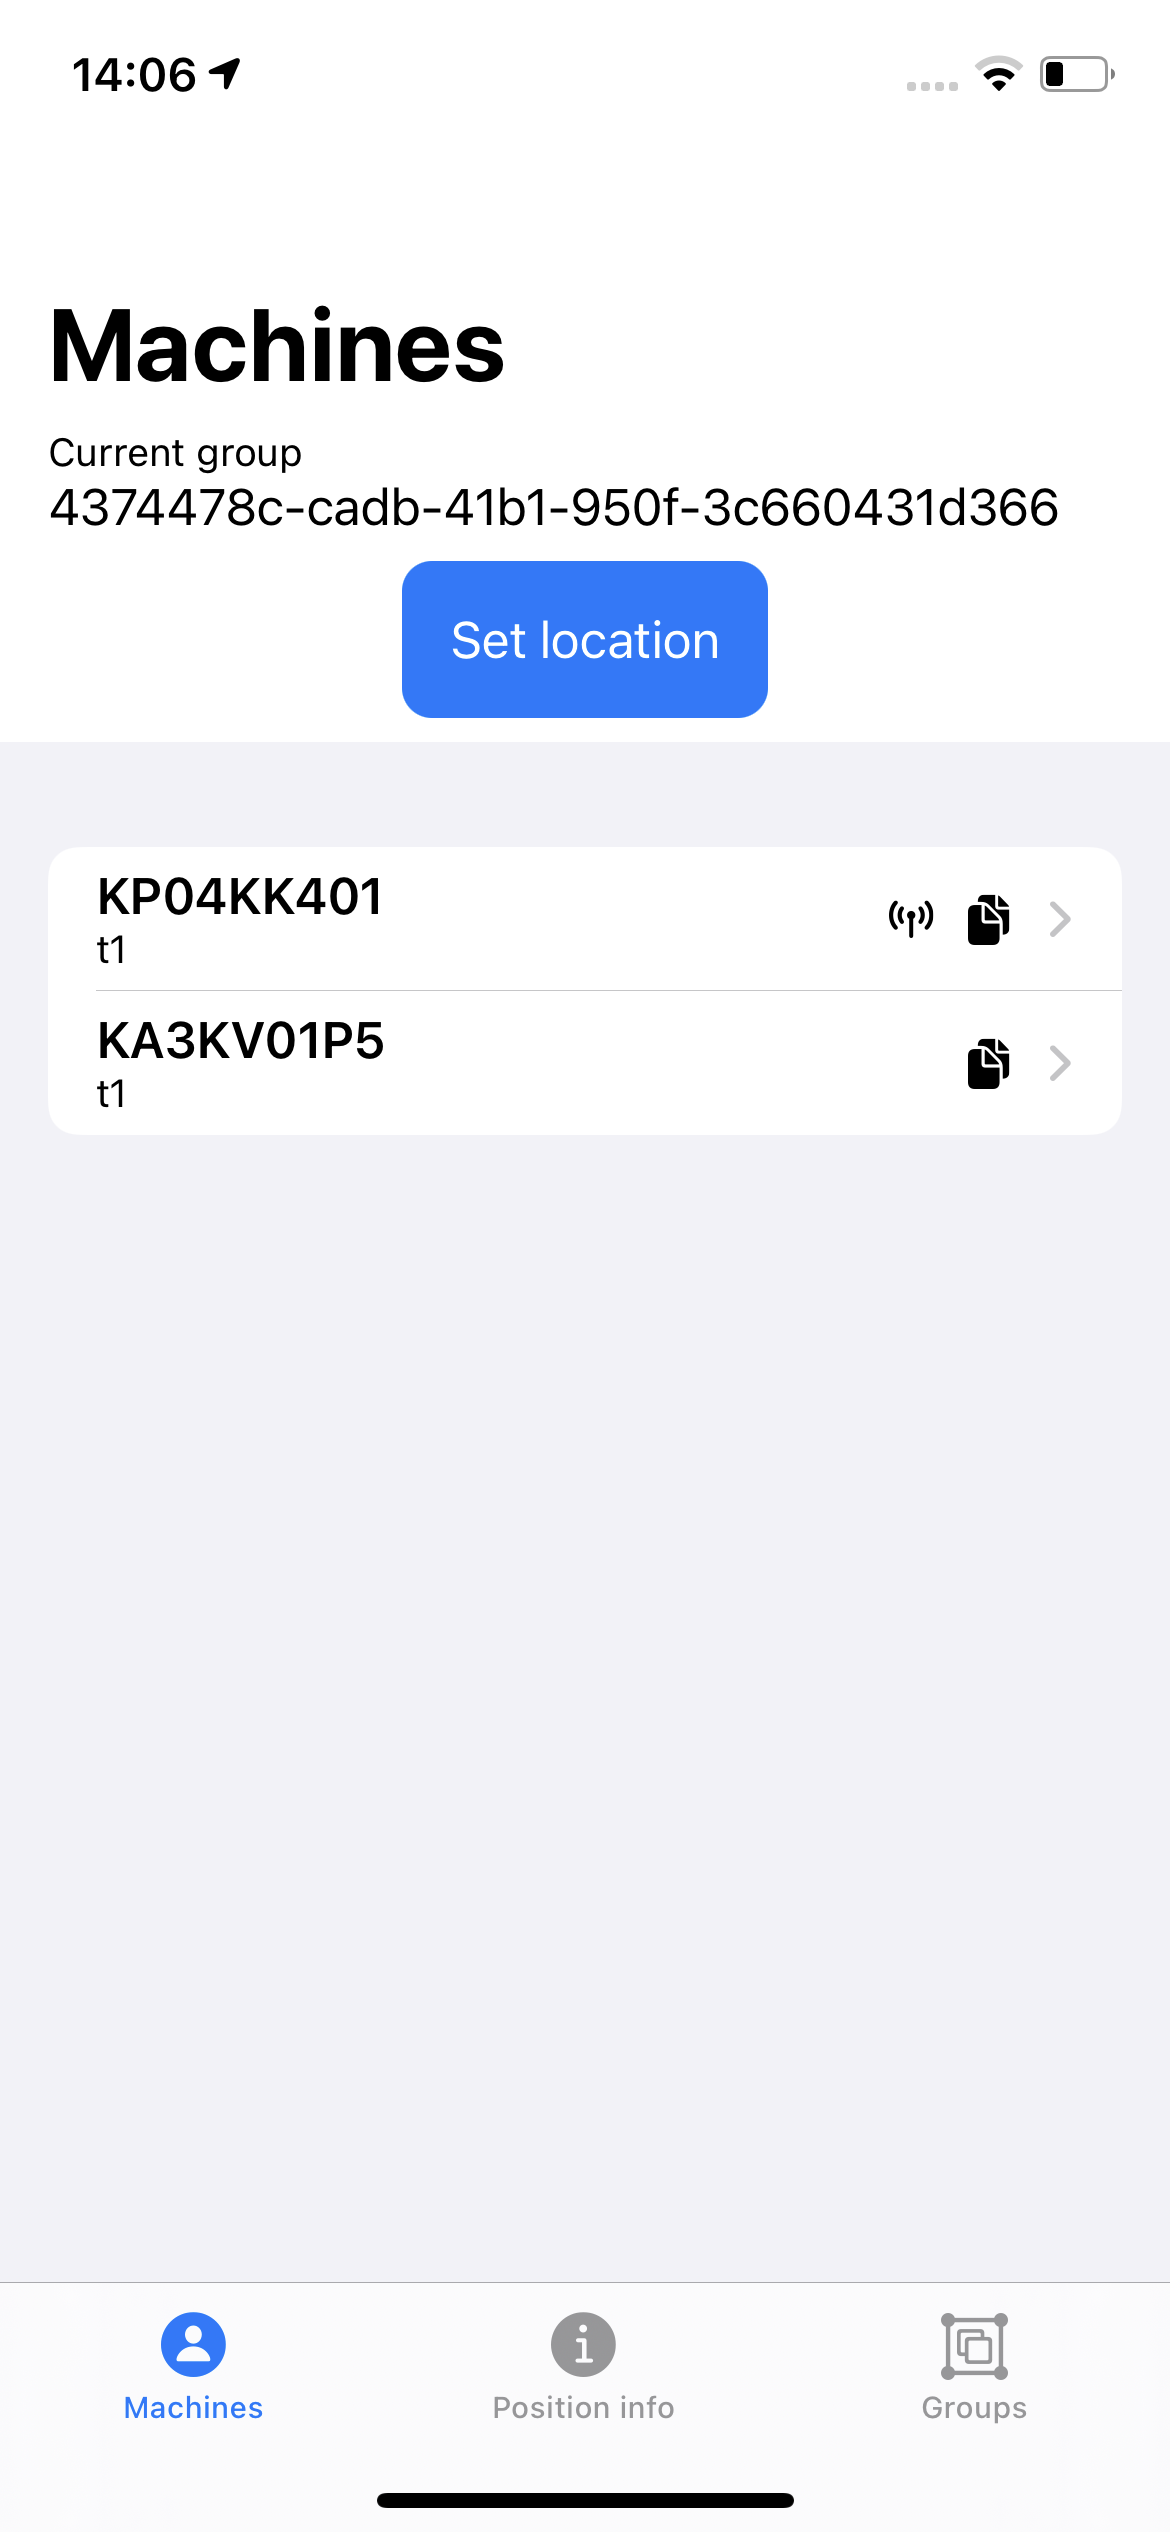
\includegraphics[width=.9\textwidth]{appScreens/machinesGroup}
		\caption{Machines list}
		\label{subfig:machinesList}
	\end{subfigure}%
	\begin{subfigure}[t]{0.3\textwidth}
		\centering	
		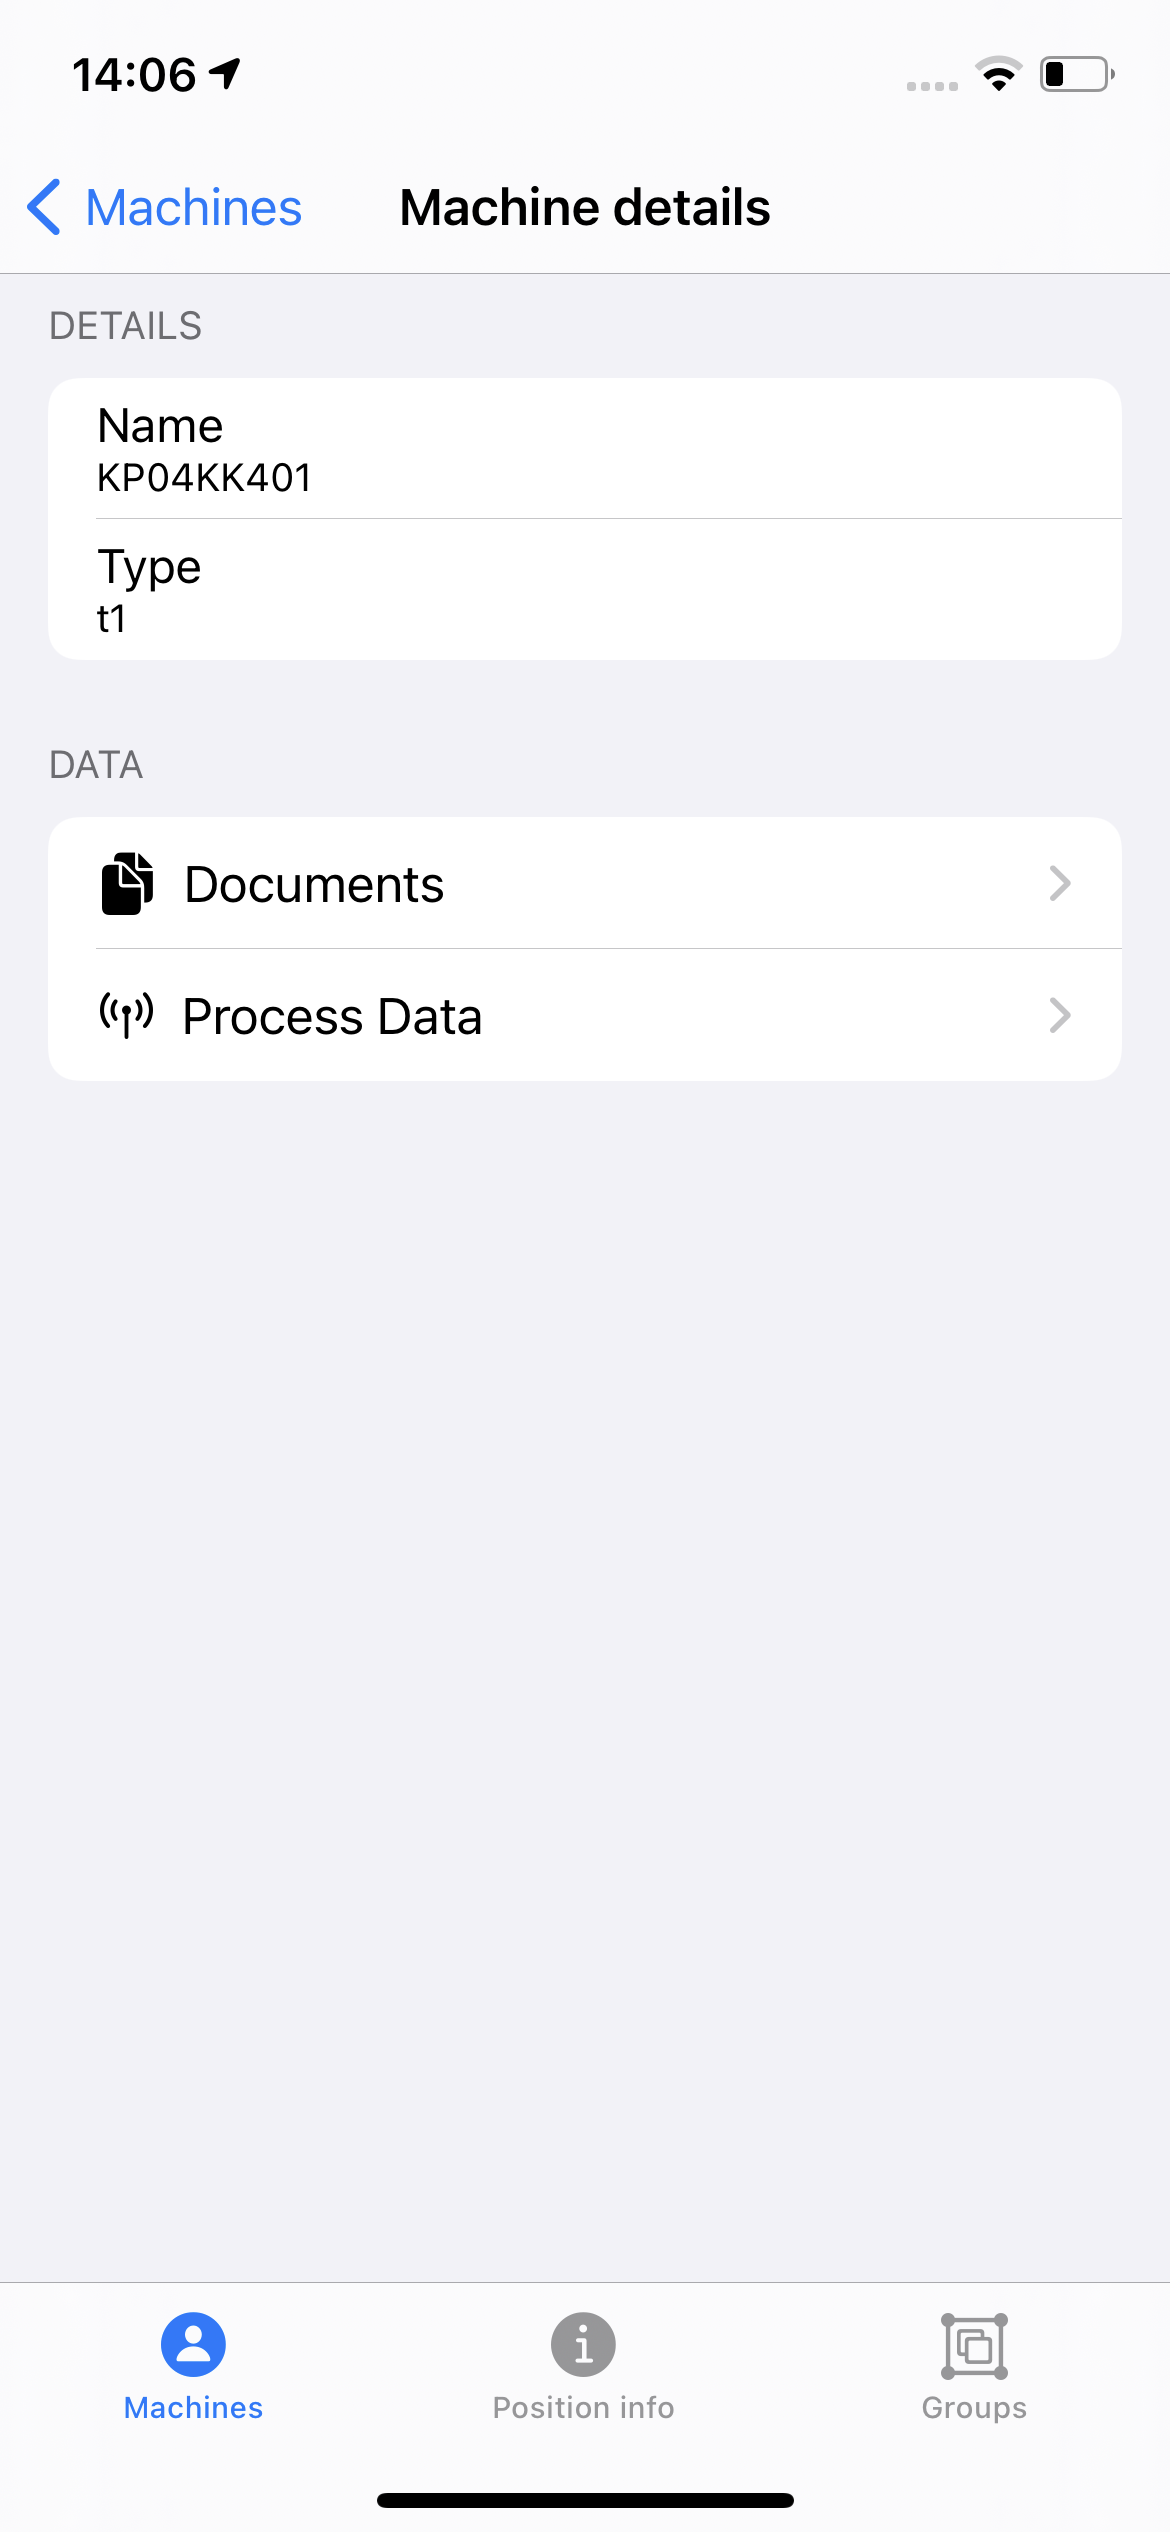
\includegraphics[width=.9\textwidth]{appScreens/machineDetails}
		\caption{Machine details}
		\label{subfig:machineDetails}
	\end{subfigure}
	\begin{subfigure}[t]{0.3\textwidth}
		\centering	
		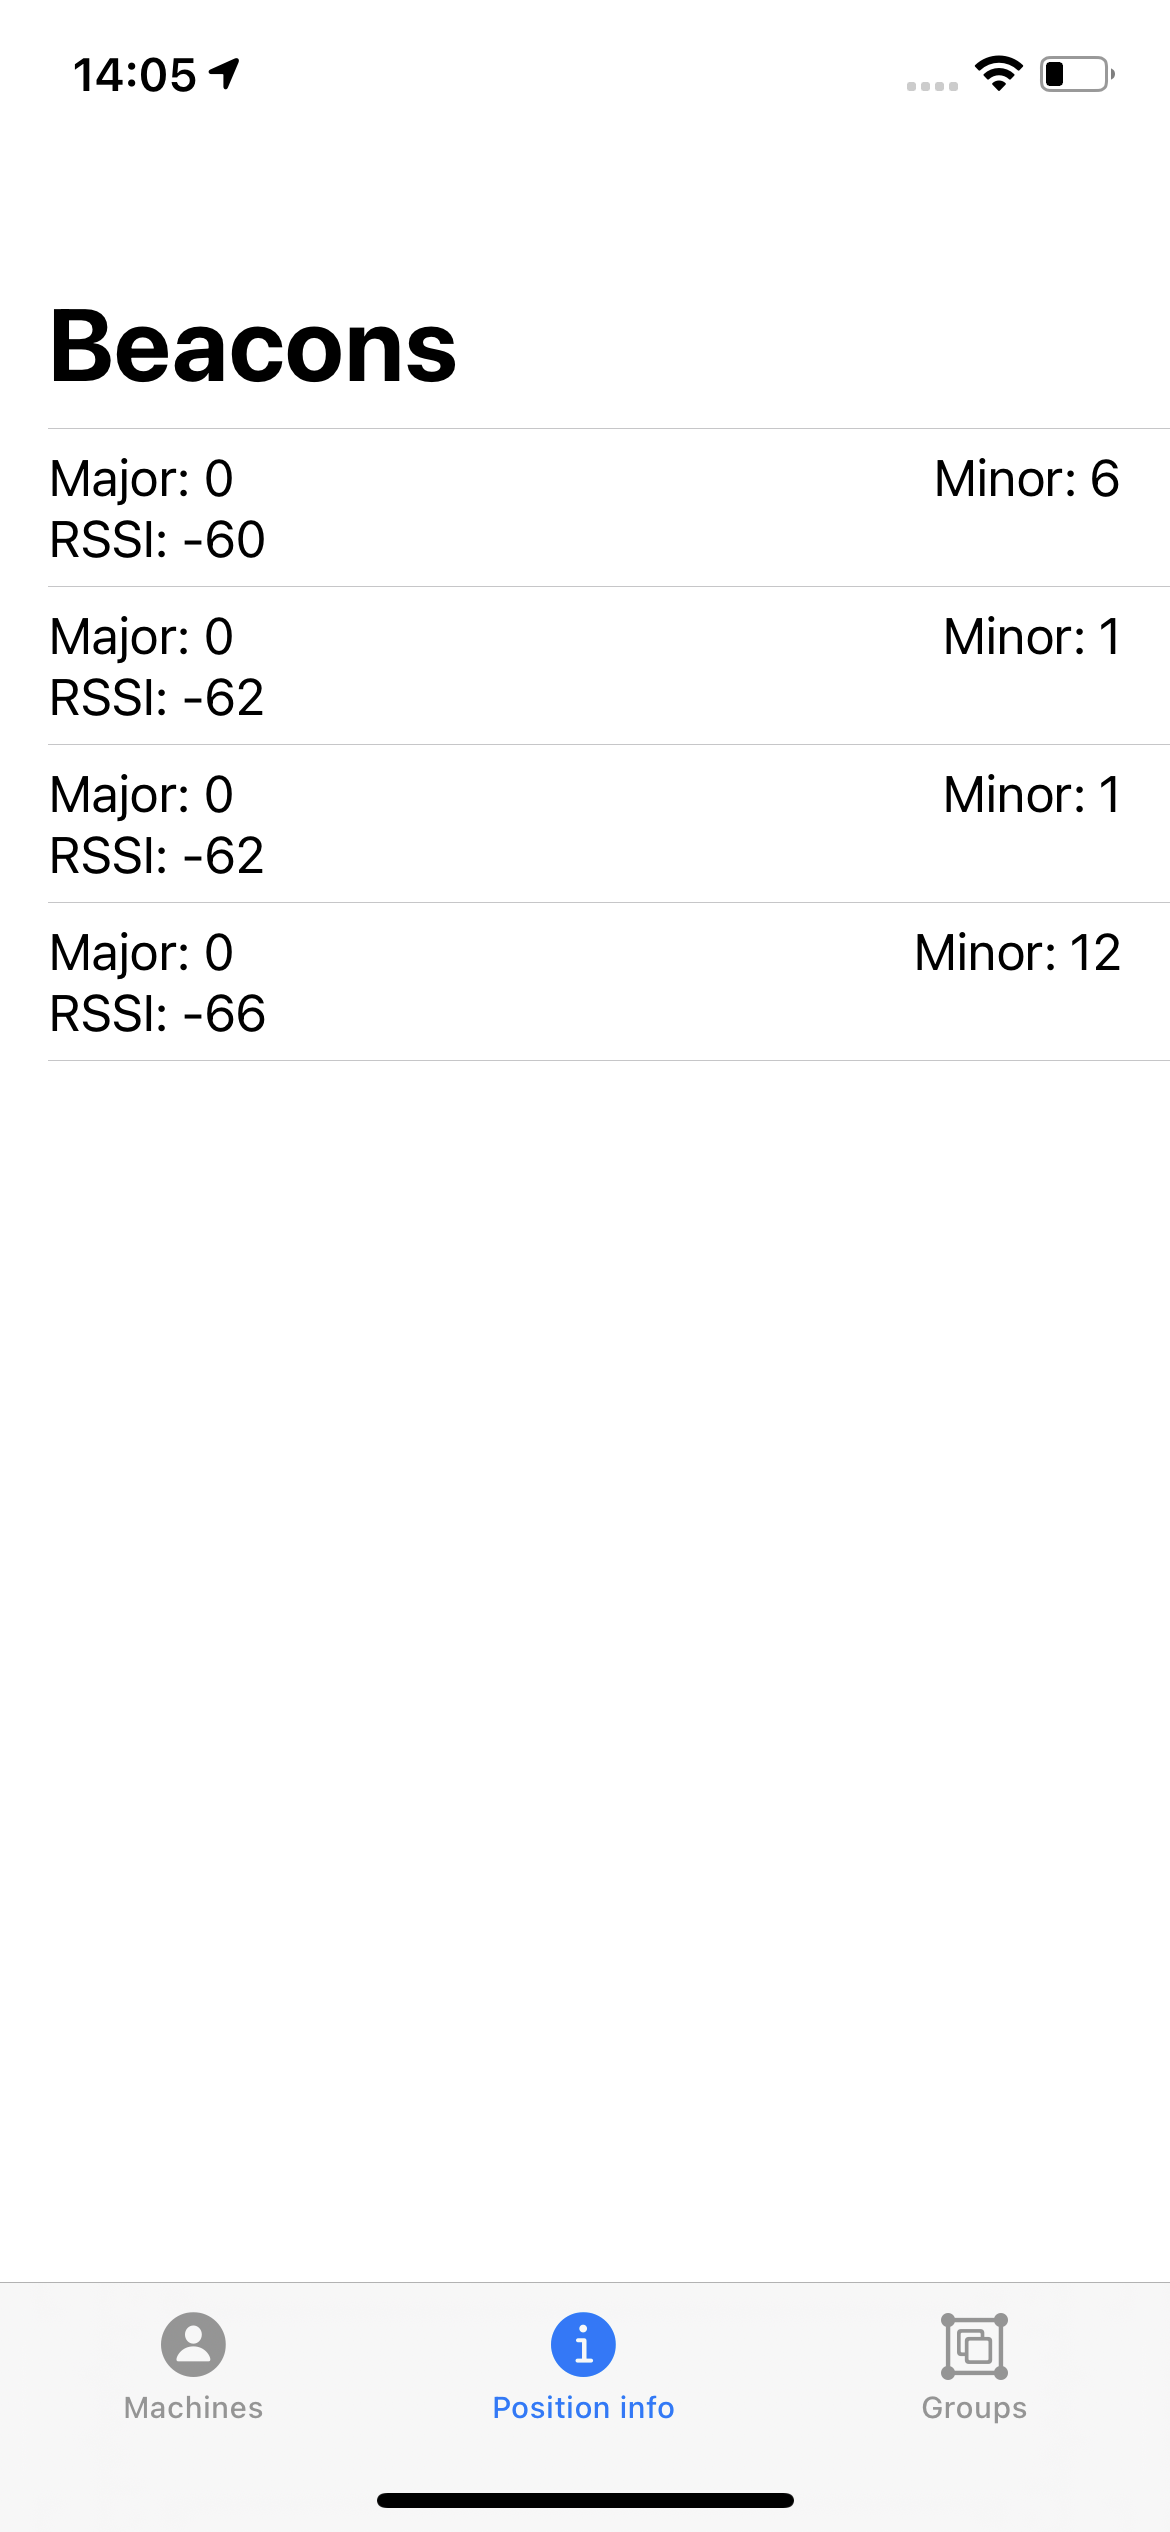
\includegraphics[width=.9\textwidth]{appScreens/beacons}
		\caption{Nearby beacons}
		\label{subfig:nearbyBeacons}
	\end{subfigure}
	\begin{subfigure}[t]{0.3\textwidth}
		\centering	
		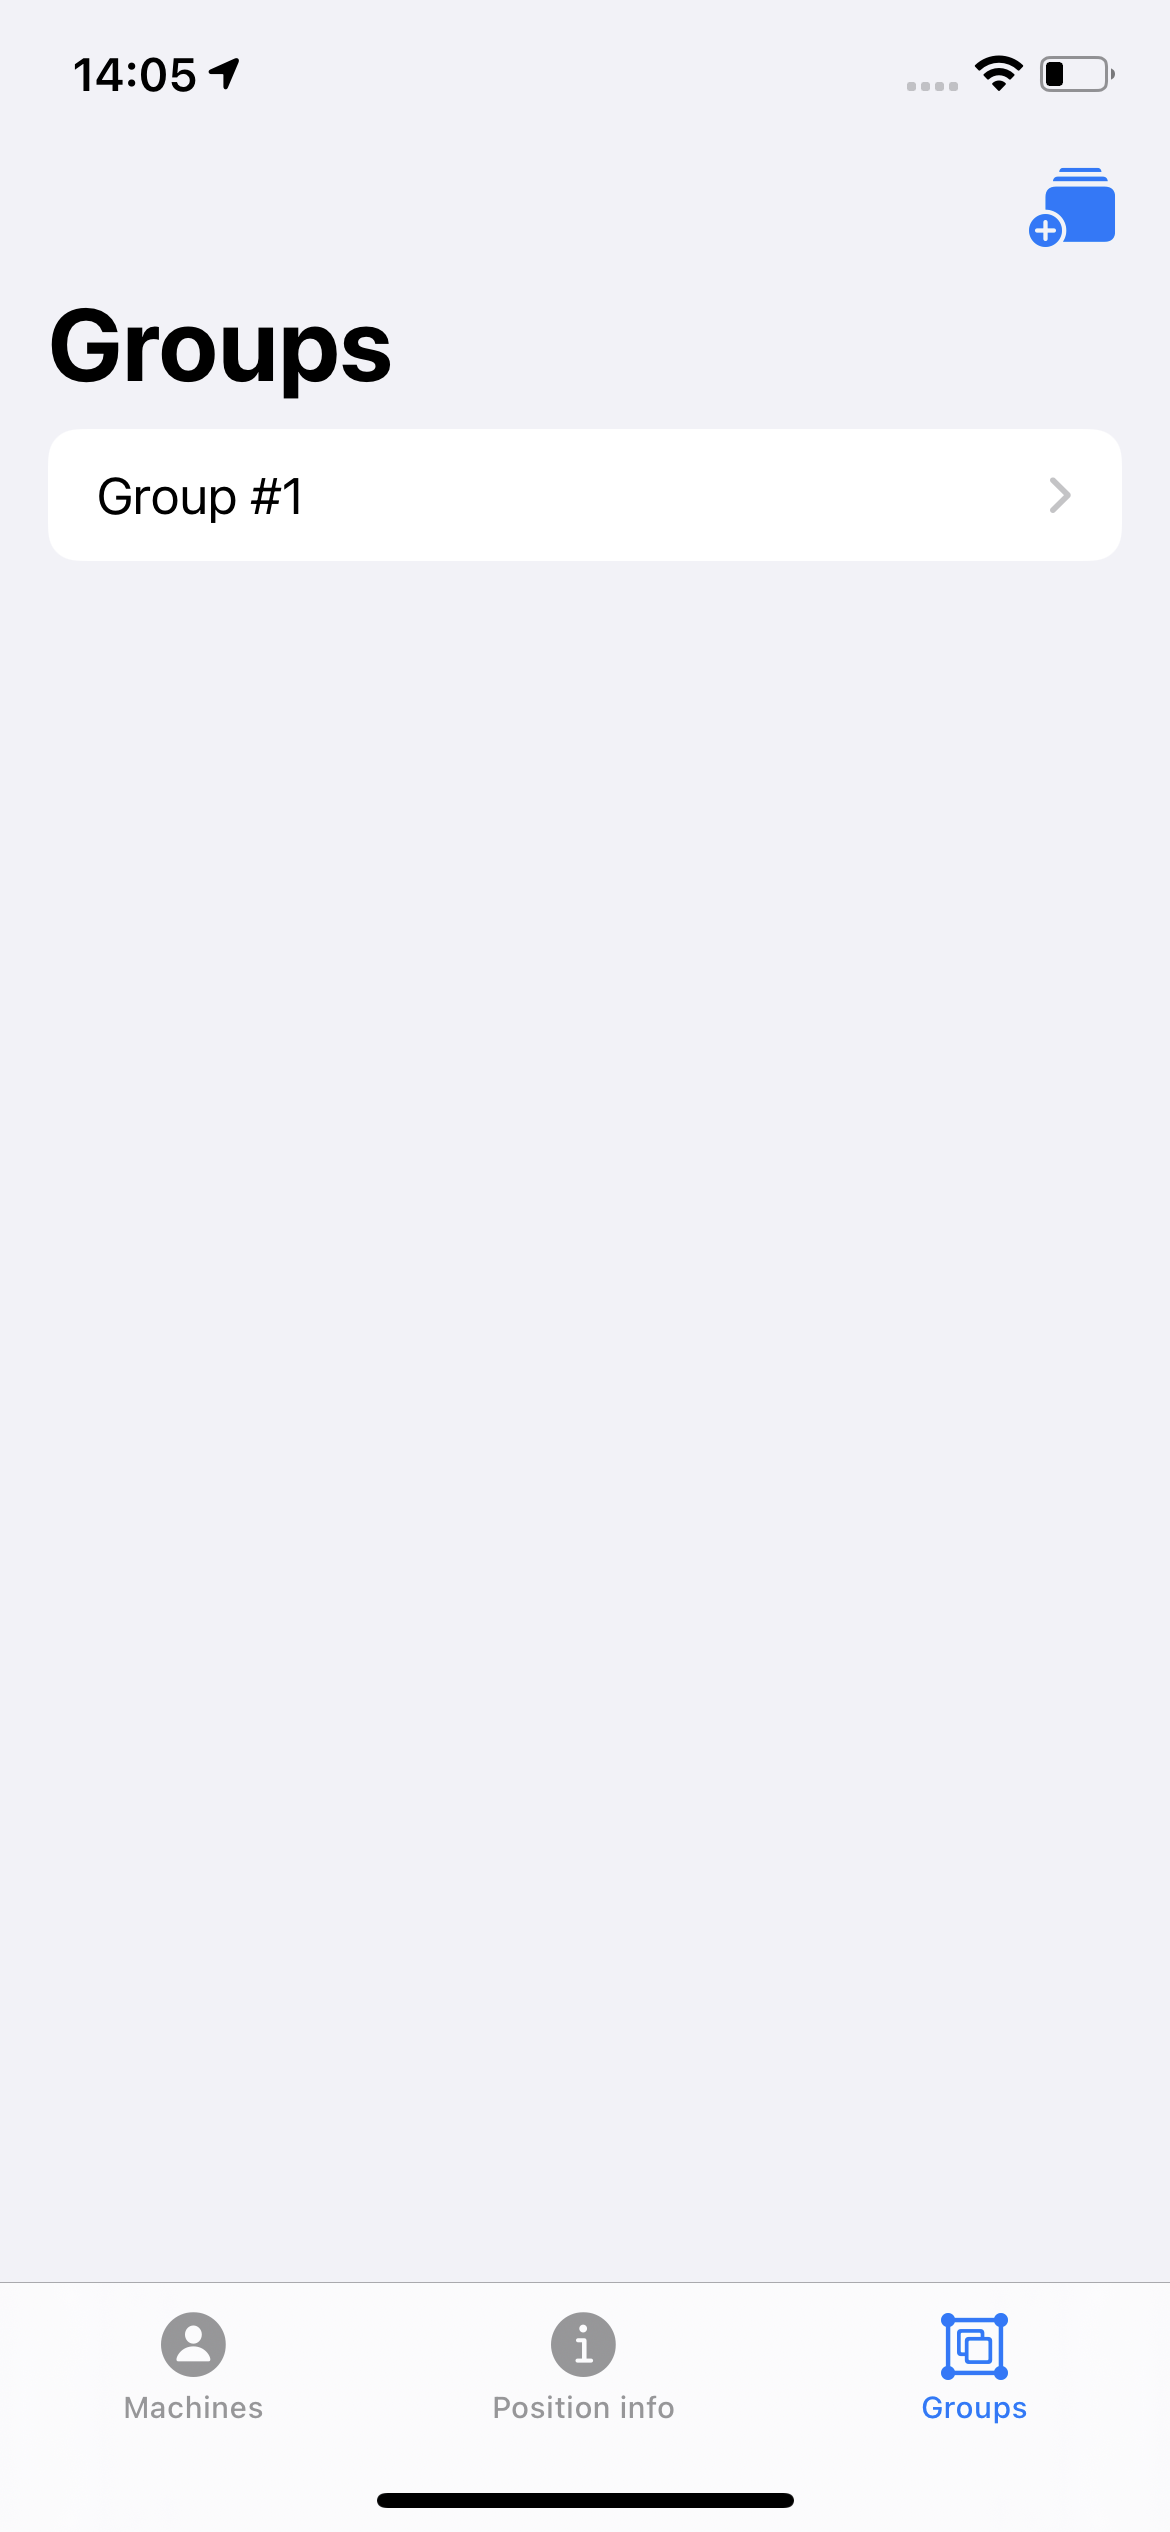
\includegraphics[width=.9\textwidth]{appScreens/groups}
		\caption{Existing groups}
		\label{subfig:existingGroups}
	\end{subfigure}
	\begin{subfigure}[t]{0.3\textwidth}
		\centering	
		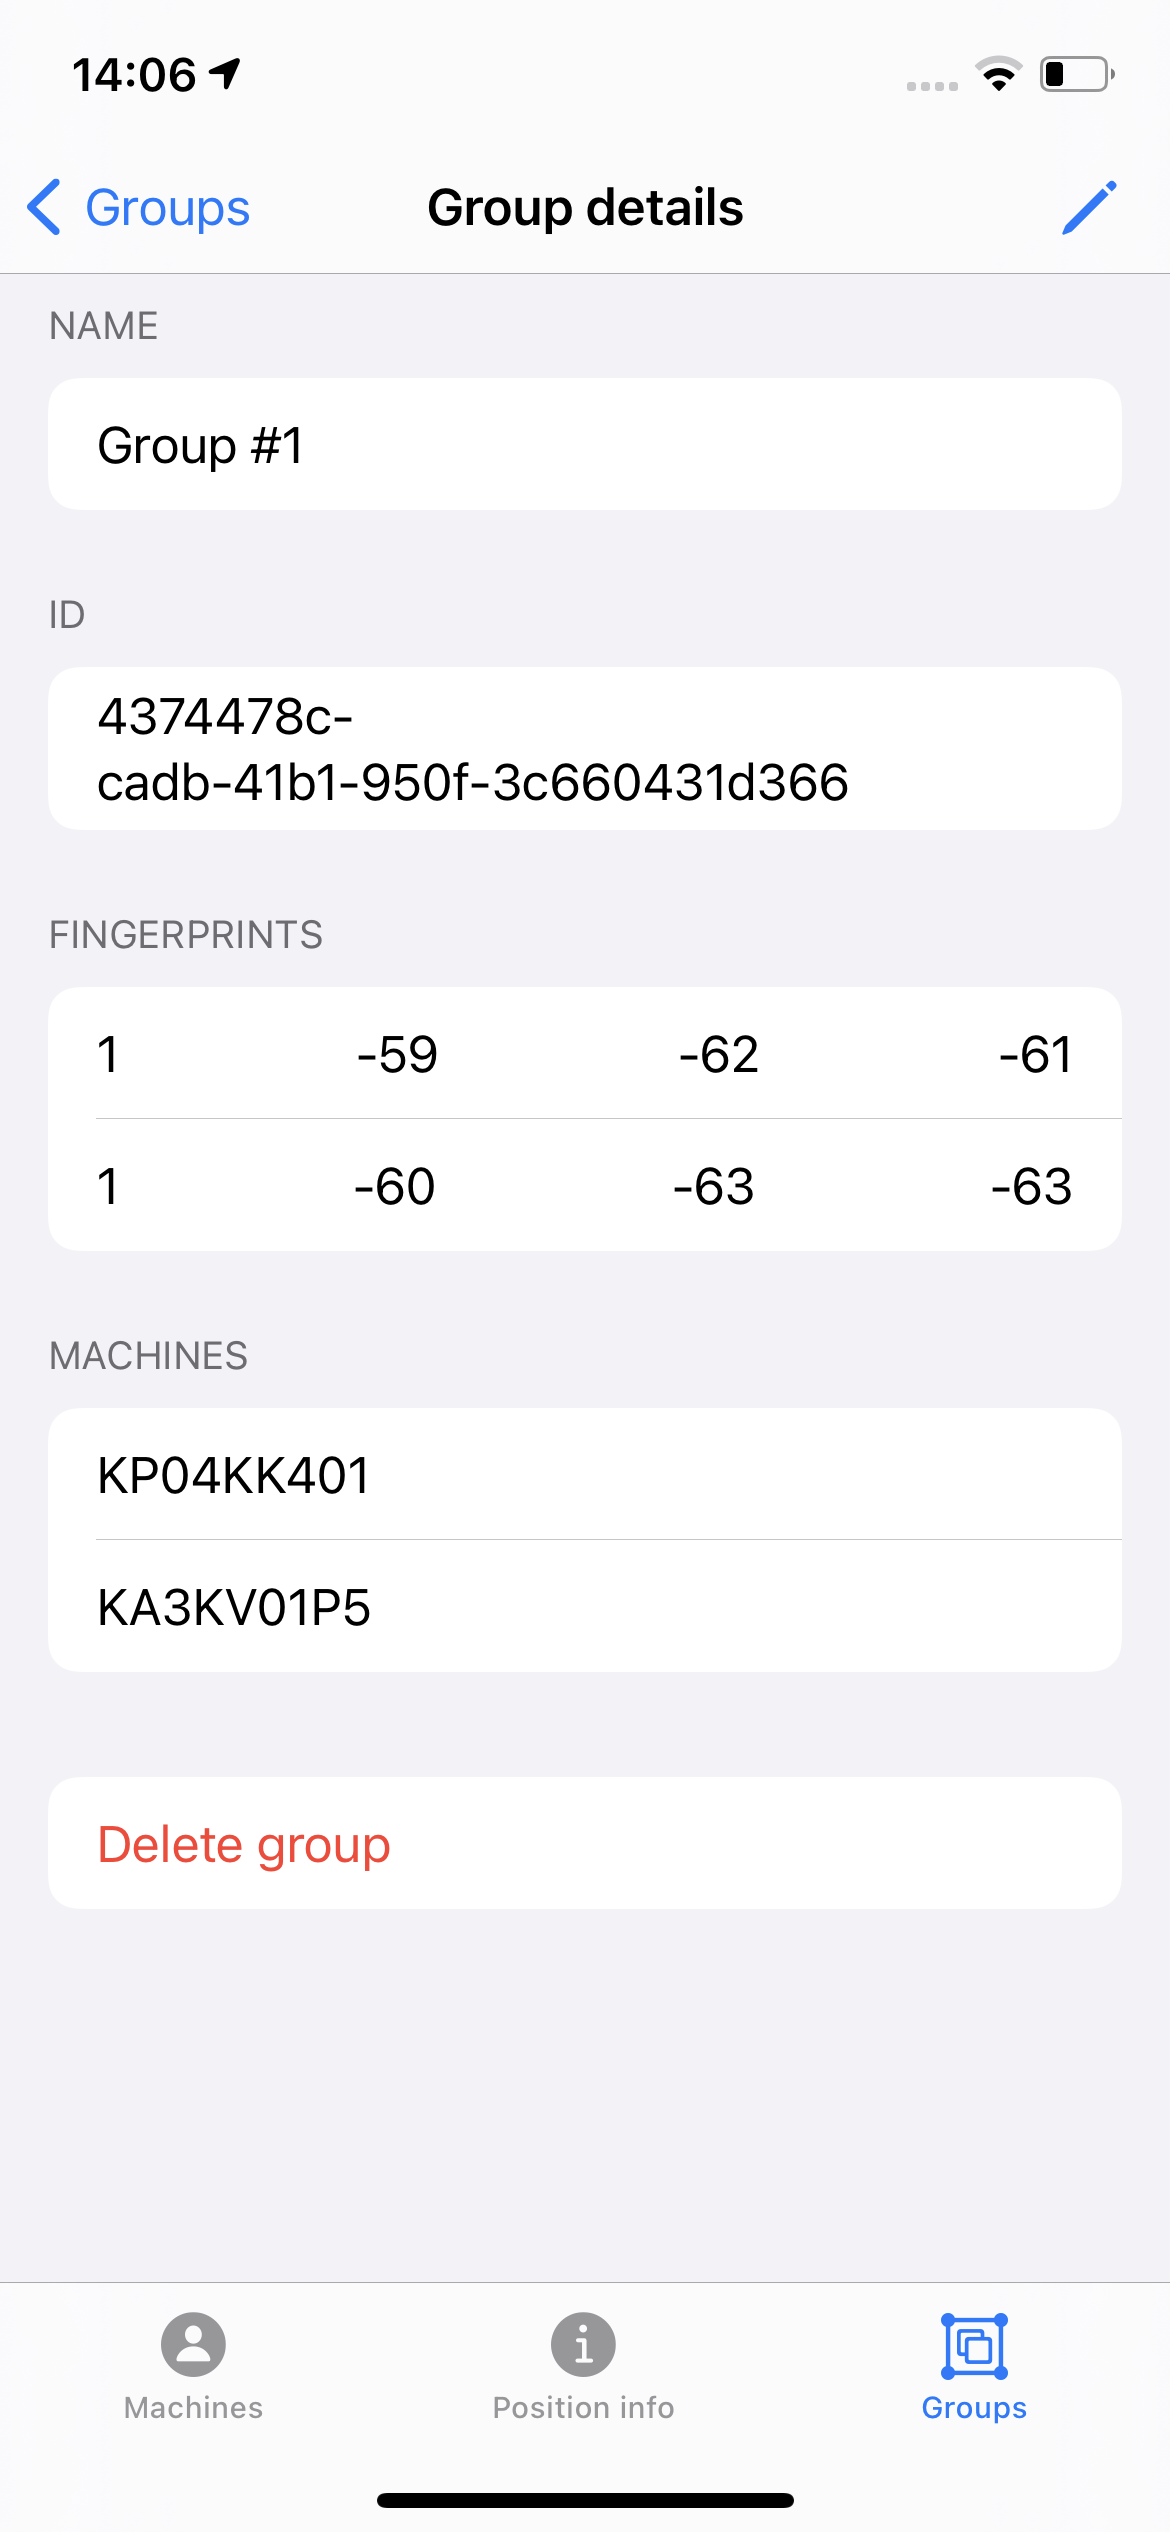
\includegraphics[width=.9\textwidth]{appScreens/groupDetails}
		\caption{Group details}
		\label{subfig:groupDetails}
	\end{subfigure}
	\begin{subfigure}[t]{0.3\textwidth}
		\centering	
		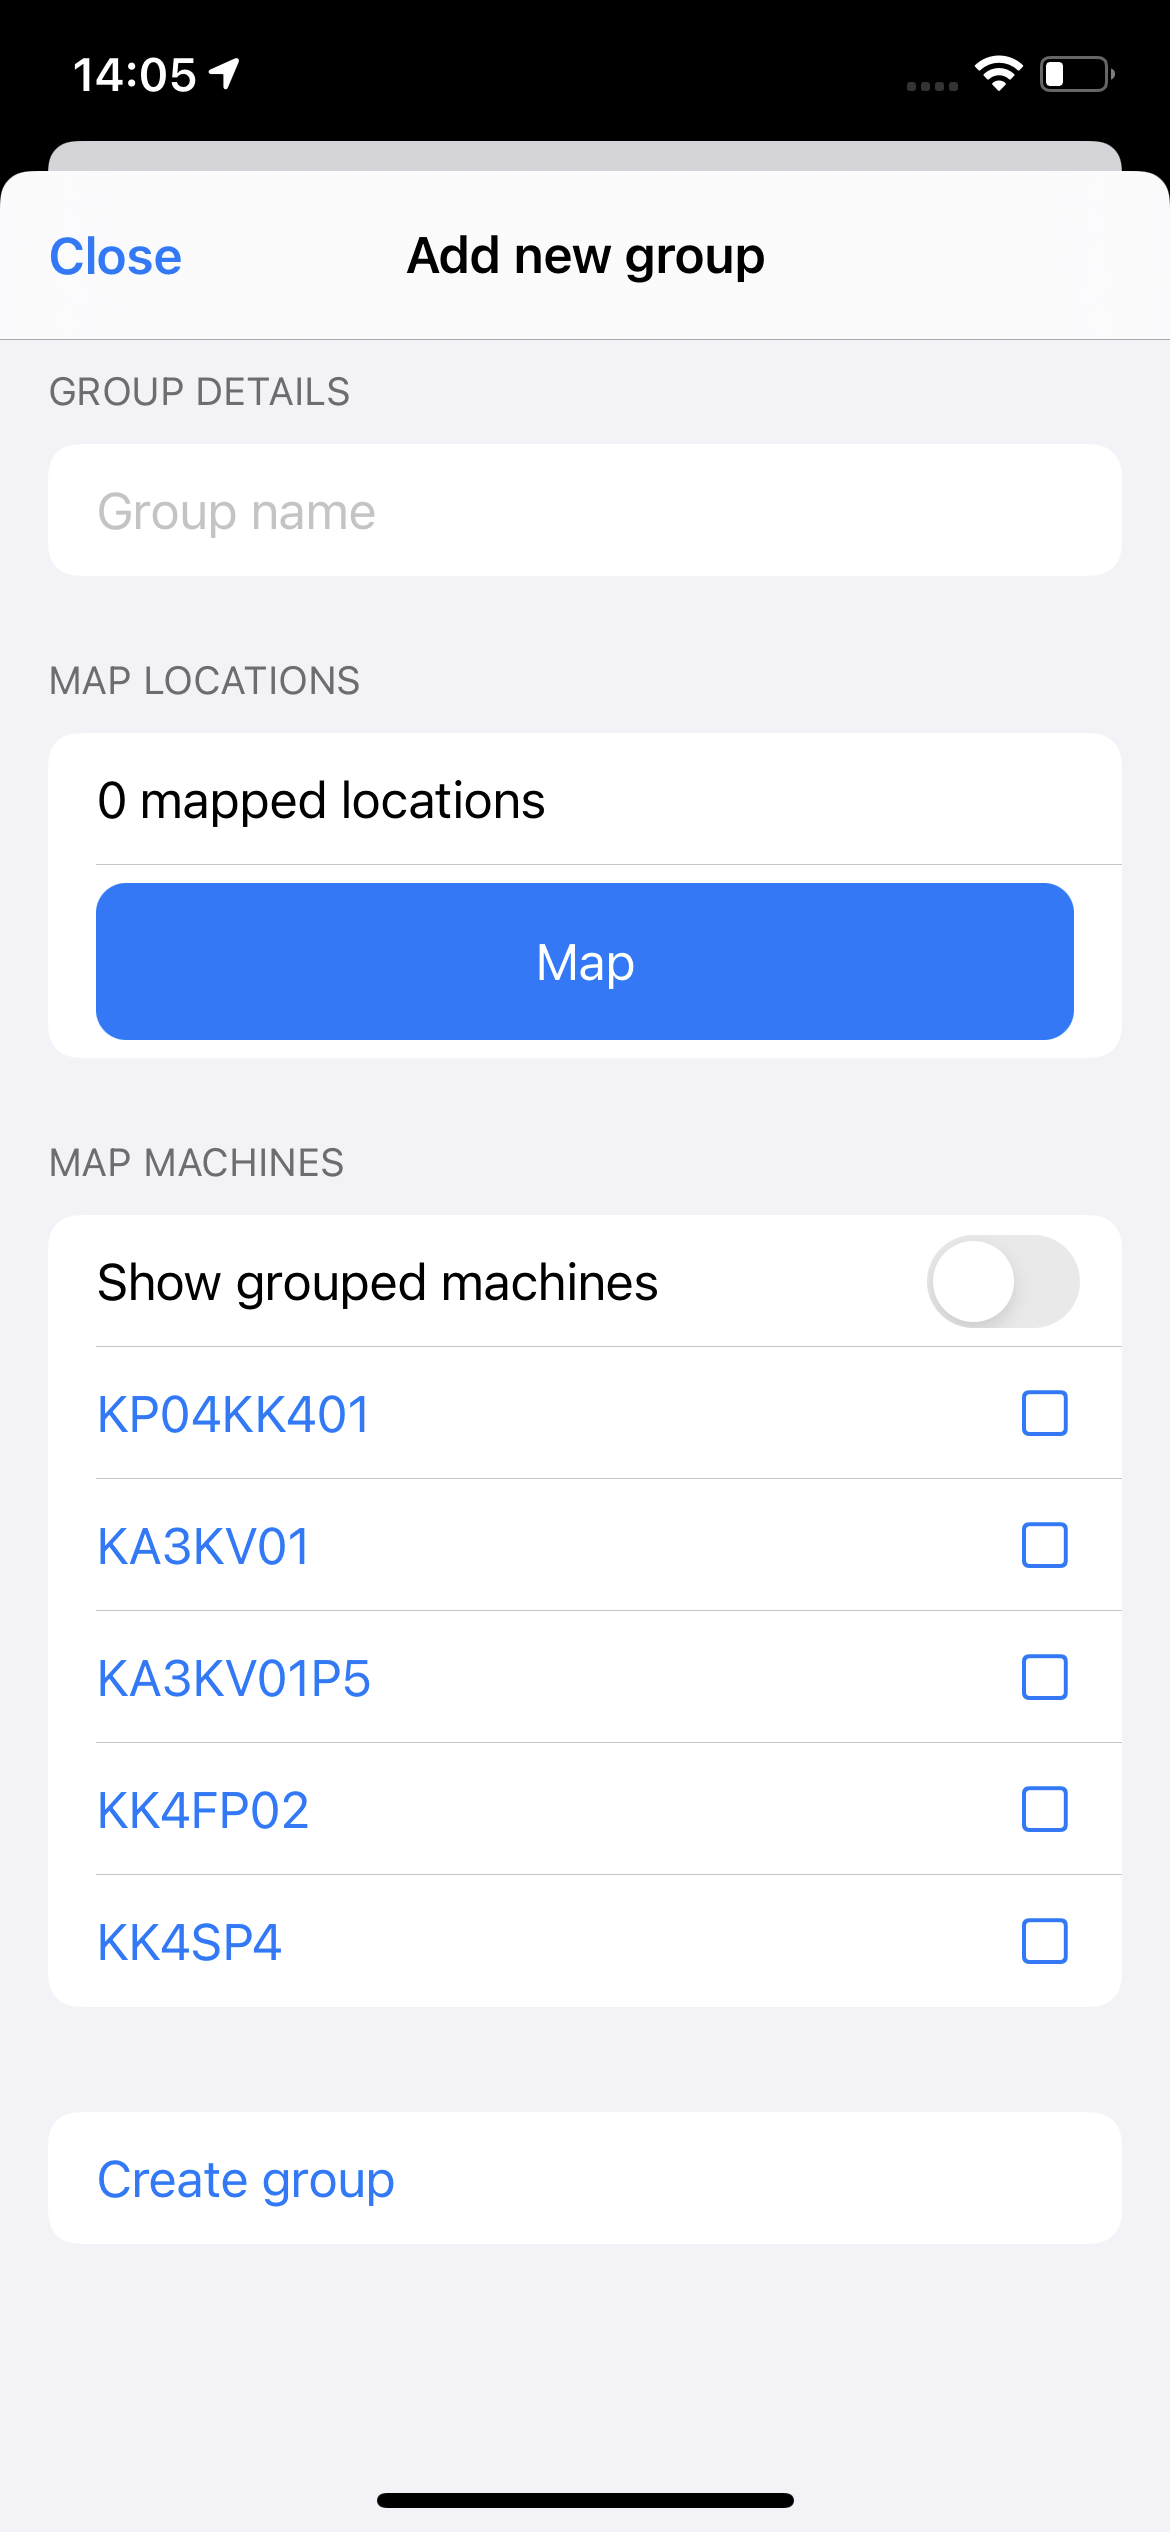
\includegraphics[width=.9\textwidth]{appScreens/newGroup}
		\caption{New group}
		\label{subfig:newGroup}
	\end{subfigure}

	\caption{Application screens}
	\label{fig:appScreens}

\end{figure}

In \Cref{subfig:machinesList} the result of the application screen to set a position and show the corresponding machines is being presented.
\Cref{sec:implAppSetPos} describes technical details how machines is being presented when a position is set.

\bigskip

\Cref{subfig:machineDetails} present the application screen to look at the details for a machine.
This screen is meant to present the documents and real time process data for a selected machine, which is not being done in this thesis. 

\bigskip

\Cref{subfig:nearbyBeacons} present a screen that shows all nearby beacons with its value that the application can read.

\bigskip

In \Cref{subfig:existingGroups} all created groups is being presented.
From this screen the details about a group can be viewed, presented in \Cref{subfig:groupDetails}.
Another feature is to create new groups within the application, which is being presented in \Cref{subfig:newGroup}.
How new group feature is implemented is being described in \cref{sec:implAppNewGroup}.

\section{Positioning}\label{sec:resultPos}
The positioning test is conducted in two steps and the condition for these are being explained in \cref{sec:methodSoftwareTests}.

\bigskip

\Cref{fig:twoVsFour} presents the accuracy of the testing for each group with one fingerprint/point and four fingerprints/point, as well as the overall accuracy.

\fig{Total accuracy per group for one and four mappings}{twoVsFour}{1}{results/twoVsFour}

As seen in \Cref{fig:twoVsFour}, the accuracy of four fingerprints (75\%) is higher than one fingerprint (44\%).
These differences are a result of how well the system can predict the location of the device.
With one fingerprint/point the position is sensitive to signal changes, since there is only one mapped fingerprint at each point in the created groups.
The \acrfull{knn} classification also has fewer fingerprints to test on which will make the prediction more uncertain.

\bigskip

With four fingerprints/point the accuracy is higher, since the prediction is not as sensitive to signal fluctuation because there are more fingerprints to test against.
This means that the \acrshort{knn} classification is able to make better predictions. 


\subsection{Measurement results per point}\label{sec:resultsPosOneFingerprint}
This sub-section presents to which group each measurement has been classified.
Each point is being classified with the majority result from the three test sets, where each set had ten measurements for each point in each group.
In the presented results the measurements for one fingerprint per point and four fingerprints per point is being compared.
See \cref{sec:methodEvaluation} for more information about this.

\bigskip

Each group has its own name as the correct group to be positioned in.
\Cref{fig:bluePointsResult} present the result for the blue group, \Cref{fig:yellowPointsResult} the yellow group and \Cref{fig:brownPointsResult} for the brown group.
The result presented in these figures shows that the group prediction with one fingerprint per point fluctuate a lot.
This has to do with that only one fingerprint is stored for each point.
Because of this the signal is sensitive to fluctuation of the \acrfull{rssi} signals from the beacons and has problems to predict the correct groups.

\bigskip

With four fingerprints the results is more stable and makes more correct predictions.
This is because the fluctuation doesn't make as big impact because of the more fingerprints for each point.

\fig{Measurement result per point for blue group}{bluePointsResult}{1}{results/pointsBlue}

In \Cref{fig:bluePointsResult} it's shown that the blue group does get predicted most of the time for both one and four fingerprints/point.
It's also shown that the brown group is almost never predicted.
This can be explained by the location of the yellow group, which is closer than the brown group.
Between the area of the blue group and the yellow and brown there was a large concrete wall.
Beacons far away would be more affected by going through this wall than nearby beacons would, which is the case for the yellow group.

\bigskip

In the cases where the yellow group is being predicted it can be explained by the beacons placement.
At certain points beacons far away from the blue group, and closer to the yellow groups, has a clear line of sight.
A result from this is that nearby beacons have a weaker signal than beacons far away.
This explanation is true for both one and four points since the beacons has the same arrangement.

\bigskip

Why the brown group get predicted at all has its explanation in signal fluctuation.
If the signal of nearby beacons fluctuates a lot it will make a false prediction, that can be of a group further away.

\fig{Measurement result per point for yellow group}{yellowPointsResult}{1}{results/pointsYellow}

In the yellow group the fluctuation is low with the majority calculated groups which is shown in \Cref{fig:yellowPointsResult}.
This is a result of a more open space where the signals are not being reflected by any walls, as well as more beacons are in range with a clear line of sight, which will give a better prediction accuracy.

\bigskip

Since the brown and yellow group is close to each other minor fluctuations in the \acrshort{rssi} signals can cause the \acrshort{knn} classification to predict the wrong group in some cases, as seen in \Cref{fig:yellowPointsResult}.

\fig{Measurement result per point for brown group}{brownPointsResult}{1}{results/pointsBrown}

In the predicted points for the brown group presented in \Cref{fig:brownPointsResult} the result is not as self explaining.
As seen in the figure, the blue group get predicted at two points.
This has to do with similar \acrshort{rssi} values of the beacons, where beacons near the blue group, and beacons in or near the brown group has similar values.
A result from this makes the prediction more unstable with the different mapped fingerprints in the groups.

\bigskip

With one fingerprint/point the prediction is only correct in the first point.
This has the same explanation as in the beginning of this sub-section, that the \acrshort{rssi} values can fluctuate so much that the outcome of the prediction changes.
The prediction is stabilizing with four fingerprints/point because there is more data to predict against, and signal fluctuations doesn't have as large impact.


\chapter{Discussion} \label{discussion}
This chapter presents the discussion around this thesis project.
It starts with a discussion about the implemented \acrfull{ips} in general.
Following this the implementation of the Apple iOS application and the server is being discussed, which then leads to the result and is being topped of with ethical and social aspects.


\section{Indoor Positioning System}\label{sec:discussionIps}
An implementation of an \acrshort{ips} is the core of this thesis work.
By developing an \acrshort{ips} application indoor positioning is possible without any GPS signals.
To develop an advance and complex application without any form of backend is in most cases not a good idea, since the system gets locked down to the chosen platform.
If a new platform going to be implemented into the system the application would need a lot of work because of its complexity.
It would also means a higher cost since it takes longer time to develop.
A backend based system would reduce the application complexity and make the adoption for new platforms easier.

\bigskip

When it comes to \acrshort{ips}'s itself it's mature enough to be implemented in real scenarios.
There is some obstacles with these systems such as positioning accuracy and the requirements to keep the system updated with both maintained hardware and radio maps.
The \acrshort{ips} in this thesis work was a \acrfull{poc} application to show the possibilities with a system like this, and how it can be implemented.
The environment where this system will be implemented and used is in large industrial environments.
These environments are changing form time to time and means that new site surveys need to be carried out to keep the radio map updated.
This is factors to take into consideration when implementing a system like this.


\section{Application development}\label{sec:}
Since the developed application was a \acrshort{poc} application some functionalities has been left out by purpose.
The application has no security against the developed backend server, which would need to be implemented in a real production application.
This to protect the API's from unauthorized access and make sure the data transmitted between the server and devices is safe.

\bigskip

Also, some parts of the application is not needed in a production state, accept for power users and admins.
These functions are the ability to create new groups and to control which beacons that are being catched by the application.
If these functions would be available for a regular user they could cause some significant damage that would need to be fixed.
A user could for example delete a group by accident.
The deleted group would then need to be recreated again with all its work. 

\bigskip

The developed user interface that's presented in the result is a good start.
It does however need some more work to make a better user experience and to show relevant information.


\section{Server development}\label{sec:}
Just like the application the server contains some parts that would not be necessary in a production environment.
Also some parts of the server is neither best practice or optimized.

\bigskip

When a position is being set by a user in the application the server would be called and return the position with help of \acrfull{knn}.
This \acrshort{knn} algorithms is being trained at every new request to the localization endpoint.
If this would be implemented in a real production this would not be suitable solution.
The \acrshort{knn} should only be trained if there is any changes to the existing data, such as a new group or additions to a already existing one.
But in testing purpose where new groups was created often this approach was necessary.

\bigskip

When the different endpoints in the server is called the server will download data from the Azure Cosmos Database every time. 
This could be avoided to instead cache all or some of the data.
This would save money in the long run since each request against Azure is a cost.


\section{Test results}\label{sec:discussionResult}
As presented in \cref{sec:resultPos} the test showed that four fingerprints per point gave the highest accuracy.
When there is only one fingerprint per point the measurement for that point will get unstable because of signal fluctuation.
This means that the point only has one value to relate to, except its neighbours, when \acrshort{knn} does its prediction.
In the case where each point has four fingerprints \acrshort{knn} foremost has more data to predict against.
But it can also accept fluctuations in the \acrshort{rssi} values when positioning, since there is more fingerprints to compare against.
The results also shows that even when a point is being scanned far away from another group the prediction can be wrong and locate the group far away.
This does mostly depend on the fluctuates of the \acrshort{rssi} signals from the iBeacons, but also how the signal is being interfered but different obstacles.

\bigskip

Other works done in the area showed that a high accuracy is hard to achieve with a \acrshort{ips}.
To be able to get a high accuracy a stable signal is a very important factor.
With \acrshort{ble} beacons, which are low powered devices, the signal can fluctuates a lot because of its limited power.
If it does the positioning can be affected, which was shown by the accuracy in this thesis result.
Related work that was investigated show that an implementation of a Kalman filter will make the prediction of the positioning better and more accurate since the unstable \acrshort{rssi} signals is being smoothed out.
It was also shown in the relates work that they got a higher accuracy than in this project.
This can depend on the model of Beacons used, differences in the implemented systems and the testing setup.
The most of these related work did test in an open environment such as a large hall or library.
In these environments there is less obstacles that can affect the \acrshort{rssi} signals.

\bigskip

The area where the tests was being conducted cannot really be used as a guidance how well a \acrshort{ips} works.
Since it differs so much from the real environments where this technique would be used.
The best suitable solution for testing is to perform these in the right type of industrial environments, which was not possible in this thesis due to the Covid pandemic.
The results does however gives a pointing finger what to be expected in terms of accuracy in a \acrshort{ips}.


% \section{Project method}\label{sec:discussionMethod}
% The used method in the project has been straightforward and general for any kind of software project.


% The method used in the project has been a good choice, since it did keep it simple to follow a set path.
% Since the method was also used by all papers presented in the related work it was a good method for a work of this kind.
% In the used approach, that was to first read about the subject and the implement a system form already known methods and tools, a structured work could be conducted.


% \section{Scientific discussion}\label{sec:discussionSientific}


\section{Ethical and social aspects}\label{sec:discussionAspects}
In a positioning system ethical aspects is always important.
Technically a positioning system that use positioning data from the device can be used to track the end users.
If the developed system run all calculations on-device this is not an issue, since no data leaves the device.
But with a system where data is sent to a remote server this is a consideration.
If these positions is mapped to a x,y-coordinate the user can be positioned and therefore surveillance of the users can be implemented.
With this in mind it's always important to inform the users what kind of data that is being used and in which way.

\bigskip

With the developed \acrshort{poc} application this is not an issue since the fingerprints are not being mapped against a coordinate.
The application can therefore be used with a good security policy that the users can trust.
On the other hand the application uses localization functions that might be possible to be used in the other way.
A sender might snap up that a specific device is connected to it and can track the user that way.
Since protecting the end users is always a high demand and makes up for a good security the system needs to be secured in good ways.
This includes the communication between the device and the server, so the connection cannot be eavesdropped and sensitive positioning data used by third parties, which would then interfere with GDPR.

\bigskip

The developed system is this project does also affect social aspects in some manner.
To maintain a system like this that need constant maintenance there will always be a trade-off between benefits and cost.
If a person going to maintain the systems this person will be a cost that is involved with the operation of the system.


\chapter{Conclusion}\label{conclusion}
This chapter presents a summary and conclusion of the projects work that start with a project summary.
This is followed by the validity of the project and ends with some thought about the future work for this project.


\section{Project summary}\label{sec:conclusionProjectSummary}
Knowledge has been gathered how an \acrfull{ips} works, according to goals \ref{goal:fieldInvestigation}, which made the goal fulfilled.
With this knowledge a \acrshort{ips} could be designed to met goal \ref{goal:systemDesign} which then would be implemented.

\bigskip

To be able to met goal \ref{goal:poc} a working \acrshort{ips} needed to be implemented in a \acrfull{poc} Apple iOS application which has been done.
This goal has therefore been met successfully.

\bigskip

To see how well the implemented \acrshort{ips} and the \acrshort{poc} application performed the system needed to be tested.
With this test the performance could be evaluated, which means that goal \ref{goal:systemEvaluation} has been met.

\bigskip

This means that all goals in this thesis project has been fulfilled with a good result.

\bigskip

The projects statement that was set at the beginning of the project has also been able to be fulfilled.
Firstly the statement is answered in the motivation of the design choices made (\cref{sec:methodSoftwareDesign}) and lastly the \acrshort{poc} application implemented in \cref{impl} showed how this was done.


\section{Project validity}\label{sec:conclusionProjectValidity}
The validity of the project can be set to class two out of a total of three.
So it's at a intermediate level with the following explanation.

\bigskip

Due to the way the tests was performed the results form them can give a pointing finger how the implemented system works.
Fully knowledge about this would be to test the system in a real industrial environment that has both the larger areas as well as the industrial obstacles.
Only then could the accuracy and the real result be seen in a full picture.

\bigskip

When it comes to the implemented system it could be implemented in a real production scenario with some more work, which is being described in \cref{sec:conclusionFutureWork} below.


\section{Future work}\label{sec:conclusionFutureWork}
\Acrlong{ips} has a bright future and is a technology that will be adopted more and more in the future.
The result the \acrlong{poc} application developed in this thesis work is in its simplest form.
LKAB will probably use this technology and continue to research and test in the area of indoor positioning.
So, this means that a future work on this work is possible and has a chance of be adopted in real production environments.

\bigskip

In the developed application security is not taken into consideration between the device and the server.
Here a better security and signing of devices that only belong to LKAB is a large part that need to be implemented.
The positioning itself could also be refined to better and more accurate position the device. 
But to achieve this the application first need to be tested in a real environment to evaluate how to continue the development.

\bigskip

Another part that would need to be refined is the presentation of the created groups.
If the application going to be used the number of groups would be large.
So to have all groups visible at all time would be a bad user experience.
Here the groups should be filtered depending on which plant and building the device is located in.
This could be done with the major value from the iBeacons.

\bigskip

When creation a new group the same problem would occur.
All machines available will make a huge list that would be hard to search in.
Here the beacon major value could also be used to filter out the relevant machines.

\bigskip

When it comes to the server this could also be further developed in some places.
How the request is made to the Azure Cosmos Database should be overseen to avoid high bills form Azure.
Also the training of \acrlong{knn} should also be done only when new groups is created.


\printbibliography

\begin{appendices}
\chapter{Requirements specification}\label{appendix:requirements}
\begin{itemize}
\item Be able to position a cellphone in indoor environments without GPS signal
\item Display data on a mapped location in a smartphone application
\end{itemize}


\chapter{New group data output}\label{appendix:newGroupData}
\fileListingNoCap{json}{newGroupData.json}



\chapter{App screens}\label{appendix:appScreens}

\end{appendices}

\end{document}
